\section{Supplementary results}
\label{sec:appendix}
This appendix collects the secondary displays referred to in the results: the moderate ratio $\rho=10$, per-split effects, rank-group recall, per-class recall, and the validation-only probe diagnostics.

\begin{table}[h]
  \centering
  \footnotesize
  \begin{tabular}{lccc}
    \toprule
    & Virchow2 & UNI2-h & UNI2-h $-$ Virchow2 \\
    \midrule
    \tabinput{tab_decomposition_10.tex}
    \bottomrule
  \end{tabular}
  \caption{At $\rho=10$ the two encoders lose almost the same accuracy on both datasets. Damage components in balanced-accuracy points with paired 95\% intervals.}
  \label{tab:decomp10}
\end{table}

\begin{table}[h]
  \centering
  \footnotesize
  \setlength{\tabcolsep}{4pt}
  \begin{tabular}{lcccccc}
    \toprule
    & \multicolumn{2}{c}{B} & \multicolumn{2}{c}{R10} & \multicolumn{2}{c}{UNI2-h $-$ Virchow2} \\
    \cmidrule(lr){2-3}\cmidrule(lr){4-5}\cmidrule(lr){6-7}
    & Virchow2 & UNI2-h & Virchow2 & UNI2-h & at B & in damage R10$-$B \\
    \midrule
    \tabinput{tab_probability_R10.tex}
    \bottomrule
  \end{tabular}
  \caption{Probability quality at $\rho=10$, in the layout of Table~\ref{tab:prob}. UNI2-h's raw ECE on TCGA-UT falls from B to R10 because its raw balanced probabilities are underconfident.}
  \label{tab:prob10}
\end{table}

\begin{table}[h]
  \centering
  \footnotesize
  \begin{tabular}{llccccc}
    \toprule
    & & \multicolumn{2}{c}{BA of B (\%)} & \multicolumn{2}{c}{$D_R(100)$ (draw SD)} & \\
    \cmidrule(lr){3-4}\cmidrule(lr){5-6}
    Dataset & Split & Virchow2 & UNI2-h & Virchow2 & UNI2-h & $\delta_R$ \\
    \midrule
    \tabinput{tab_splits.tex}
    \bottomrule
  \end{tabular}
  \caption{The TCGA-UT damage reduction appears in every split; the BRACS splits disagree. Observed per-split means over ten draws, with the standard deviation of $D_R$ across draws in parentheses.}
  \label{tab:splits}
\end{table}

\begin{table}[h]
  \centering
  \footnotesize
  \begin{tabular}{llcccccc}
    \toprule
    & & \multicolumn{3}{c}{Virchow2} & \multicolumn{3}{c}{UNI2-h} \\
    \cmidrule(lr){3-5}\cmidrule(lr){6-8}
    Dataset & Third & B & R100 & Change & B & R100 & Change \\
    \midrule
    \tabinput{tab_thirds.tex}
    \bottomrule
  \end{tabular}
  \caption{On TCGA-UT UNI2-h keeps more tail recall at $\rho=100$; on BRACS both encoders collapse the tail. Mean test patient-macro recall (\%) of the head, body, and tail thirds of classes by their assigned rank in each draw.}
  \label{tab:thirds}
\end{table}

\begin{figure}[h]
  \centering
  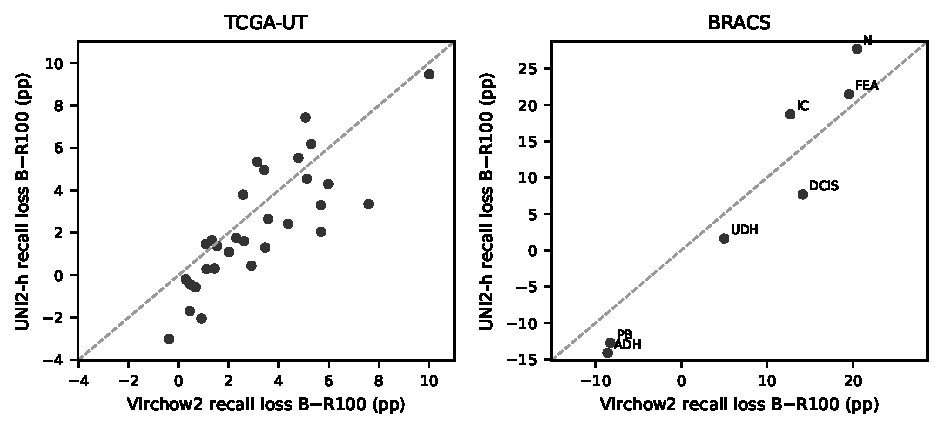
\includegraphics[width=0.85\textwidth]{fig_per_class.pdf}
  \caption{Most TCGA-UT classes lose less recall with UNI2-h; BRACS classes scatter on both sides of the diagonal. Each point is one class's recall under B minus its recall under R100, averaged over all 30 draws and therefore over the ranks the class visits; points below the dashed diagonal lose less with UNI2-h.}
  \label{fig:perclass}
\end{figure}

\begin{table}[h]
  \centering
  \footnotesize
  \setlength{\tabcolsep}{3.5pt}
  \begin{tabular}{llcccccccccccc}
    \toprule
    & & & & \multicolumn{4}{c}{B} & \multicolumn{4}{c}{R100} & \\
    \cmidrule(lr){5-8}\cmidrule(lr){9-12}
    Dataset & Encoder & Dim. & Norm & Val.\ BA & Margin & Std. & $T$ & Val.\ BA & Margin & Std. & $T$ & Edge \\
    \midrule
    \tabinput{tab_validation.tex}
    \bottomrule
  \end{tabular}
  \caption{Validation-only probe diagnostics. Norm is the mean Euclidean norm of the native validation features. Val.\ BA is the selected probe's validation patient-macro balanced accuracy (\%). Margin is the mean raw logit margin of validation patches, the true-class logit minus the strongest competing logit; Std.\ divides each fit's mean margin by that fit's margin standard deviation (no fit had zero variance). $T$ is the mean fitted temperature. Edge counts selections at a grid endpoint over all seven arms and 30 fits.}
  \label{tab:validation}
\end{table}
